\chapter{Situation de départ}

\section{Contexte}
Ce chapitre a pour but de présenter l'intégralité des travaux effectués lors du précédent projet de Bachelor, réalisé par Thomas Freyche. De nombreuses images sont reprises de son rapport \cite{Freyche}.

En cas d'évolution, celle-ci sera mentionnée explicitement en fin de sous-section afin d'avertir le lecteur des modifications par rapport à la situation initiale. Dans le cas contraire, cela signifie qu'aucune modification n'a été apportée à cette partie de la maquette.

\section{Mise en place de CCS}
\label{sec:MiseEnPlace}

\subsection{Installation de Code Composer Studio}
Afin de programmer correctement le DSP, une version spécifique de Code Composer Studio (CCS) ainsi qu'une bibliothèque dédiée au DSP doivent être installées.

La version requise de CCS est la suivante \cite{CCS_Install} :
\url{https://www.ti.com/tool/download/CCSTUDIO/12.6.0} \\

Pour la bibliothèque C2000Ware, la version suivante doit être installée \cite{C2000_Install} :
\url{https://www.ti.com/tool/download/C2000WARE/5.02.00.00}\\

\subsection{Configuration de CCS}

Une fois l'installation terminée, il est nécessaire de configurer CCS pour qu'il détecte la bibliothèque. La procédure d'intégration est la suivante :

\begin{enumerate}
    \item Lancer Code Composer Studio.

    \item Accéder au menu \textit{Window > Preferences}.

    \item Dans la colonne de gauche, naviguer vers \textit{Code Composer Studio > Products}.

    \item Vérifier la liste "Product discovery path". Si le dossier \verb|C:\ti| n'y figure pas, cliquer sur \textit{Add...} et le sélectionner.
    \item Cliquer sur le bouton \textit{Refresh}.

    \item La bibliothèque C2000Ware doit apparaître dans la liste « Discovered products ». Cliquer alors sur \textit{Install}.

    \item Si l'explorateur de fichiers s'ouvre, sélectionner l'emplacement exact du dossier (généralement \verb|C:\ti\c2000\C2000Ware_5_02_00_00|).

    \item Vérifier que le dossier est correctement coché et cliquer sur \textit{Apply and close}. La figure \ref{fig:Res_conf_C2000} illustre le résultat attendu.

          \begin{figure}[htbp]
              \centering
              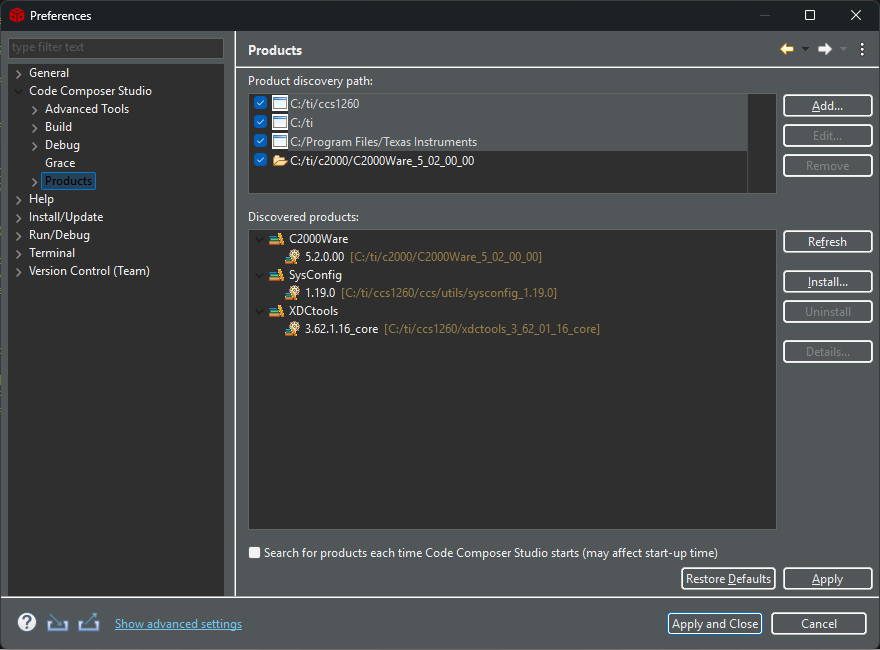
\includegraphics[width=0.75\linewidth]{Image/Chap.2/Resultat_conf_C2000.png}
              \caption{Résultat de la configuration du C2000}
              \label{fig:Res_conf_C2000}
          \end{figure}

    \item Une fois la configuration terminée, cliquer sur le bouton \textit{Build} pour appliquer les changements.
\end{enumerate}

Enfin, il est impératif de vérifier que le niveau d'optimisation de CCS est correctement établi en suivant ces étapes :

\begin{enumerate}
    \item Effectuer un clic droit sur le projet.

    \item Sélectionner \textit{Properties}.

    \item Dérouler l'onglet \textit{Build > C2000 Compiler > Optimization}.

    \item Appliquer les paramètres tels qu'illustrés dans la fenêtre suivante :

          \begin{figure}[H]
              \centering
              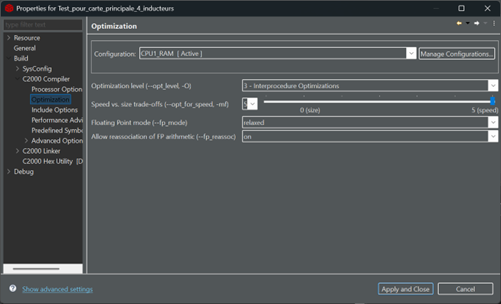
\includegraphics[width=0.75\linewidth]{Image/Chap.2/CCS_Opti_Windows.png}
              \caption{Configuration des paramètres d'optimisation}
              \label{fig:Res_conf_Opti}
          \end{figure}
\end{enumerate}

\red{Pour finaliser la mise en service, il est nécessaire de charger le programme dans la mémoire Flash du processeur.}

Il est désormais possible d'utiliser CCS pour la programmation du DSP.

\section{Protocole de mise en service}
\label{sec:Protocole}
La mise en service de la maquette s'effectue selon la procédure suivante :

\begin{enumerate}
    \item Allumer l'alimentation 48 V en réglant la limitation de courant à 3.5A. Pour ajuster cette limite, presser le bouton de réglage correspondant sur l'alimentation.

    \item Compiler et charger la dernière version du code depuis Code Composer Studio vers le DSP.

    \item Configurer l'oscilloscope sur la résistance de charge des cartes de puissance (calibres : 50 ms/div et 10 V/div pour les deux sondes). Placer le trigger du canal mesurant le côté électrique de la résistance (vers les cartes de puissance) à 20 V. Régler l'oscilloscope en mode "Single" afin d'observer la charge des condensateurs lors de l'enclenchement de l'interrupteur S1.

    \item Une fois la tension de 48 V établie et le transistor commuté, presser le bouton physique S2 ou cliquer sur le bouton \textit{Start} dans l'onglet "Mise en marche" de l'interface logicielle pour lancer la sustentation.
\end{enumerate}

\section{Hardware}
La section suivante traite l'électronique réalisée dans la version initiale du projet.

\subsection{Schéma fonctionnel}
Le schéma fonctionnel, repris du travail de Thomas Freyche, est le suivant :

\subsection{Alimentation}

\subsection{Conditionneur}

\subsection{DSP}

\subsection{ESP32}

\subsection{Test de la carte}

\subsection{PCB}

\section{Software}
Cette section traite du fichier principal (\texttt{hrpwm\_ex1\_duty\_sfo.c}) développé jusqu'à présent.

Ce fichier centralise l'ensemble de la logique de commande, notamment la régulation, l'acquisition des données ADC et la communication sans fil. Les fonctionnalités implémentées sont les suivantes :

\begin{itemize}
    \item Gestion des interruptions.
    \item Lecture de 8 canaux ADC (mesures de position et de courant par inducteur).
    \item Conversion des valeurs brutes de l'ADC en grandeurs physiques.
    \item Procédure de lancement de la sustentation.
    \item Régulation de position par retour d'état.
    \item La régulation de courant avec des régulateurs PI.
    \item Calcul des cycles de travail (PWM) en fonction de la régulation.
    \item Affectation des signaux PWM aux broches de commande du pont en H.
    \item Communication UART avec l'ESP32.
\end{itemize}

Les paragraphes suivants détaillent les différentes composantes logicielles, des bibliothèques utilisées jusqu'aux structures d'interruption.

\subsection{Algorithme du code principal}
Actuellement, l'algorithme du code principal suit la structure suivante :

\begin{figure}[H]
    \centering
    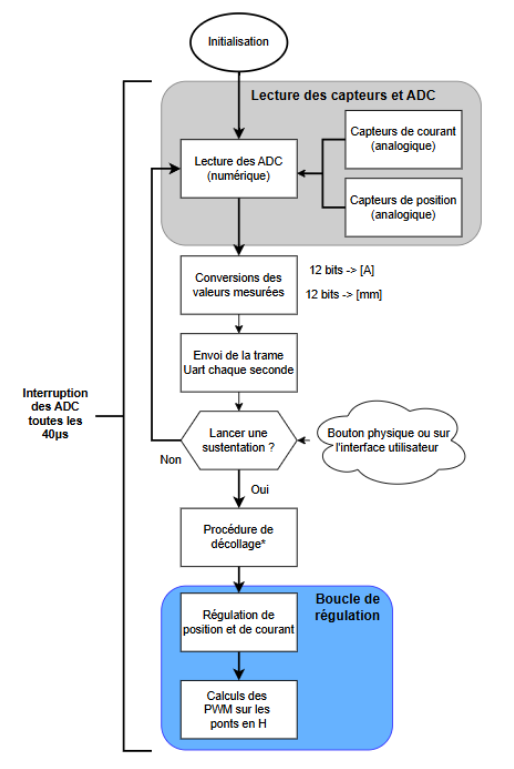
\includegraphics[width=0.7\linewidth]{Image/Chap.2/Algorithme.png}
    \caption{Structure de l'algorithme du code principal}
    \label{fig:AlgorithmeCodePrincipal}
\end{figure}

La majeure partie du code est exécutée au sein d'une routine d'interruption. Celle-ci englobe la lecture et la conversion des ADC, les algorithmes de régulation, la mise à jour des PWM ainsi que la gestion de l'interface utilisateur (bouton).

\subsection{Librairies}
Le projet s'appuie sur les bibliothèques suivantes :

\begin{minted}{c}
#include "driverlib.h"
#include "device.h"
#include "board.h"
#include "sfo_v8.h"
#include "math.h"
#include "stdio.h"
#include "FunctionHeader.h"
\end{minted}

\begin{itemize}
    \item \texttt{driverlib.h} : Bibliothèque fondamentale pour le DSP TI C2000. Elle fournit des fonctions de haut niveau permettant la configuration du matériel (\texttt{ADC\_readResult}, \texttt{GPIO\_writePin}, etc.) sans manipulation directe des registres.
    \item \texttt{device.h} : Fichier spécifique au microcontrôleur utilisé. Il définit les fonctions d'initialisation système nécessaires au fonctionnement de l'horloge et du matériel.
    \item \texttt{board.h} : Fichier généré par l'outil SysConfig (voir \ref{subsubsec:SysConfig}). Il contient les définitions des entrées/sorties configurées via l'interface graphique.
    \item \texttt{sfo\_v8.h} : Bibliothèque indispensable pour l'utilisation du HRPWM (High-Resolution PWM). Elle assure une calibration en temps réel des signaux afin de compenser les dérives thermiques ou les variations de tension.
    \item \texttt{math.h} et \texttt{stdio.h} : Bibliothèques standards C pour les opérations mathématiques et les flux d'entrées/sorties.
    \item \texttt{FunctionHeader.h} : En-tête local regroupant les définitions spécifiques à la maquette (voir \ref{subsubsec:FunctionHeader}).
\end{itemize}

\subsubsection{SysConfig}
\label{subsubsec:SysConfig}
L'outil SysConfig, accessible via le fichier \texttt{hrpwm\_ex1\_duty\_sfo.syscfg}, offre une interface graphique pour la configuration du DSP. Il est utilisé pour initialiser les modules suivants :

\begin{itemize}
    \item Les ADC.
    \item Les modules PWM.
    \item Le module de communication SCI (UART).
\end{itemize}

L'interface propose une vue schématique du microcontrôleur, facilitant la gestion du mappage des broches. Une fois la configuration validée, l'outil génère automatiquement les fichiers \texttt{board.h} et \texttt{board.c}.

\subsubsection{\texttt{FunctionHeader.h}}
\label{subsubsec:FunctionHeader}
Ce fichier regroupe l'ensemble des définitions de constantes et des prototypes de fonctions. Les éléments principaux sont :

\begin{itemize}
    \item Paramètres physiques : Caractéristiques de la maquette (entrefer, masse, inductance et géométrie des bobines).
    \item Configurations électriques : Tension du bus DC (48V) et paramètres de quantification de l'ADC (12 bits).
    \item Paramètres PWM : Fréquence de découpage (25 kHz), temps morts des MOSFET et corrections associées.
    \item Paramètres de la régulation de courant (PI) : Consigne de décollage (3A), gains $K_p$, $\tau_i$ et $G_i$.
    \item Paramètres de la régulation (Espace d'état) : Gains $K_\omega$, $K_d$ et $K_r$.
    \item Filtres numériques : Coefficients et taille de fenêtre pour les filtres IIR, FIR et Savitzky.
\end{itemize}

\subsection{Fonctions importantes}

\subsubsection{PI\_current\_regulator}
La fonction \texttt{PI\_current\_regulator} est la suivante :

\begin{minted}{c}
void PI_current_regulator(float ic, float current, float *integral,
float *ue, float *uc){
    float ie = (ic - current) * KP_I;
    *integral += (ie - *ue) * GI_I * H;
    float uc_prim = ie + *integral;

    *uc = uc_prim;
    if (uc_prim > UMAX) {
        *uc = UMAX;
    }
    if (uc_prim < 0) {
        *uc = 0;
    }

    *ue = (uc_prim - *uc) * ANTIWINDUP_EN;
}
\end{minted}

Cette fonction réalise la régulation de courant par une structure PI. Elle prend en entrée les paramètres suivants :

\begin{itemize}
    \item Le courant de consigne $ic$.
    \item Le courant réel actuel $current$.
    \item L'adresse de l'intégrale $integral$.
    \item L'adresse de l'erreur de tension $ue$.
    \item L'adresse de la consigne de tension $uc$.
\end{itemize}

Les étapes de la régulation sont les suivantes :

\begin{enumerate}
    \item Calcul de l'erreur $i_e$ entre le courant de consigne et le courant réel, puis multiplication de cette différence par le gain proportionnel du régulateur.

    \item Calcul de l'intégrale en ajoutant à la valeur précédente la différence entre l'erreur de courant $i_e$ et l'erreur de tension $u_e$, multipliée par le gain intégral $GI_I$ et la période d'échantillonnage $H$.

    \item Calcul de la tension de consigne intermédiaire ($u_{c\_prim}$) par la somme de l'intégrale et de l'erreur de courant.

    \item Vérification des limites de tension afin de ne pas dépasser les plages de fonctionnement de la maquette (entre 0 V et $U_{MAX}$ = 48 V). En cas de dépassement, la consigne est fixée à la borne correspondante.

    \item Calcul de l'erreur sur la tension par la différence entre la consigne intermédiaire et la consigne finale, pondérée par le coefficient d'anti-windup.
\end{enumerate}

Cette fonction sera principalement utilisée dans l'interruption principale pour la régulation de courant des bobines(voir \ref{subsubsec:RegCourant}).

\subsubsection{Filtre de Savitzky}
L'implémentation du filtre de Savitzky est la suivante :

\begin{minted}{c}
float savitzky_Filter(float *Buffer)
{
    float v = 0.0f;
    uint16_t m = 0;

    for(m = 0; m < FILTWINDOW; m++)
        v += F_PWM*Buffer[m]*SAVITZKY[m];

    for(m = 0; m < FILTWINDOW-1; m++)
        Buffer[m] = Buffer[(m+1)];

    return v;
}
\end{minted}

Le filtre de Savitzky \cite{Savitzky} est employé pour lisser les signaux présentant un bruit important tout en préservant la tendance de la variation du signal.

Le fonctionnement du filtre est illustré ci-dessous :

\begin{figure}[H]
    \centering
    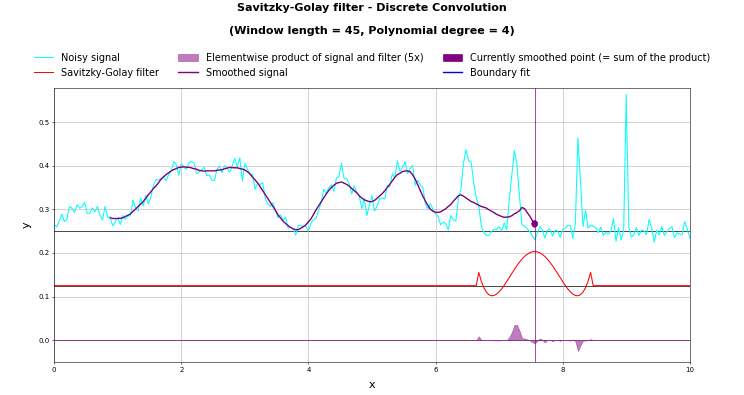
\includegraphics[width=1\linewidth]{Image/Chap.2/PrincipeSyvitzky.png}
    \caption{Principe du filtre de Savitzky}
    \label{fig:PrincipeSavitzky}
\end{figure}

Le filtre de Savitzky s'apparente à un filtre FIR à fenêtre glissante. Dans la configuration actuelle, les 9 dernières positions de l'inducteur sont conservées en mémoire. Une moyenne pondérée est ensuite calculée en multipliant chaque position par les coefficients de Savitzky correspondants :

\begin{minted}{c}
//savitzky filter coefficients, order = 2, window = 9
const float SAVITZKY[FILTWINDOW] = {-0.0667, -0.05, -0.0333, -0.0167,
                                     0.0, 0.0167, 0.0333, 0.05, 0.0667};
\end{minted}

L'augmentation de la taille de la fenêtre permet d'obtenir un signal plus lisse, mais entraîne en contrepartie une augmentation du temps de calcul.

Ce filtre est actuellement utilisé dans le code pour traiter le bruit des mesures provenant des ADC de position (voir \ref{subsubsec:ADC}).

\subsubsection{Filtre IIR}
L'implémentation du filtre IIR est la suivante :

\begin{minted}{c}
float IIR_Filter(float *entree, float *sortie)
{
    float somme = 0.0;
    float somme2 = 0.0;

    uint16_t k = 0;

    //difference equation
    for(k = 0; k < Nb; k++) //Num.
        somme += b[k]*entree[k];
    for(k = 0; k < Na; k++) //Den.
        somme2 += a[k]*sortie[k];

    //update buffers
    for(k = (Na-1); k > 0; k--)
        sortie[k] = sortie[(k-1)];

    sortie[0] = (somme-somme2);

    for(k = (Nb-1); k > 0; k--)
        entree[k] = entree[(k-1)];

    return (somme-somme2);
}
\end{minted}

Ce filtre possède une structure de type coupe-bande. Son objectif est d'atténuer une fréquence parasite apparaissant aux alentours de 75 Hz. Actuellement, l'origine exacte de ces perturbations n'est pas déterminée, mais leur filtrage est nécessaire pour assurer la stabilité de la régulation.

\subsection{Main}
Le programme principal s'exécute au sein de la fonction \texttt{main} suivante :

\begin{minted}{c}
void main(void)
{
    //
    // Initialize device clock and peripherals
    //
    Device_init();

    //
    // Disable pin locks and enable internal pull ups.
    //
    Device_initGPIO();

    //
    // Initialize PIE and clear PIE registers. Disables CPU interrupts.
    //
    Interrupt_initModule();

    //
    // Initialize the PIE vector table with pointers to the shell Interrupt
    // Service Routines (ISR).
    //
    Interrupt_initVectorTable();

    //
    // Calling SFO() updates the HRMSTEP register with calibrated MEP_ScaleFactor.
    // HRMSTEP must be populated with a scale factor value prior to enabling
    // high resolution period control.
    //
    while(status == SFO_INCOMPLETE)
    {
        status = SFO();
        if(status == SFO_ERROR)
        {
            error();   // SFO function returns 2 if an error occurs & # of MEP
        }              // steps/coarse step exceeds maximum of 255.
    }

    //
    // Disable sync(Freeze clock to PWM as well)
    //
    SysCtl_disablePeripheral(SYSCTL_PERIPH_CLK_TBCLKSYNC);

    //
    // Initialize the EPWM GPIO Pins, the SCI and change the XBAR inputs from using GPIO0
    //
    Board_init();
    SCI_enableInterrupt(mySCI0_BASE, SCI_INT_RXFF); // Autorise l'interruption Rx

    //
    // Enable sync and clock to PWM
    //
    SysCtl_enablePeripheral(SYSCTL_PERIPH_CLK_TBCLKSYNC);

    //
    // Enable Global Interrupt (INTM) and realtime interrupt (DBGM)
    //
    EINT;
    ERTM;

    // Affection des PWMs sur les x inducteurs (en fonction de
    // NUM_OF_PWM_CHANNEL, 4 par default)
    for(i = 1;i<1+NUM_OF_PWM_CHANNEL;i++)
    {
        dutyFine = ((float)(duty_table[i]*TIME_BASE_PERIOD) * INV_FACTOR);
        count = (dutyFine * (float32_t)(EPWM_TIMER_TBPRD << 8)) * INV_FACTOR;
        compCount = (count);
        HRPWM_setCounterCompareValue(ePWM[i], HRPWM_COUNTER_COMPARE_A, compCount);
        HRPWM_setCounterCompareValue(ePWM[i], HRPWM_COUNTER_COMPARE_B, compCount);
    }

    // Extinctions LEDs
    GPIO_writePin(myLED_D1,1);
    GPIO_writePin(myLED_D2,1);
    GPIO_writePin(LED_D5_carte_principale,0);
    GPIO_writePin(LED_D6_carte_principale,0);

// Infinite loop
    for(;;)
    {

    }
}
\end{minted}

L'initialisation du microcontrôleur est effectuée par les fonctions \texttt{Device\_init} et \texttt{Device\_initGPIO} issues de la bibliothèque \texttt{device.h}.

L'initialisation des interruptions est réalisée au moyen des fonctions \texttt{Interrupt\_initModule} et \texttt{Interrupt\_initVectorTable} (définies dans \texttt{device.h}).

La boucle \texttt{while} assure la calibration du module SFO (Scale Factor Optimizer). Ce processus garantit une précision optimale des impulsions PWM.

La fonction \texttt{SysCtl\_disablePeripheral} désactive la synchronisation et gèle l'horloge des modules PWM.

La fonction \texttt{Board\_init} configure les périphériques (ADC, PWM, UART, etc.) selon les réglages établis dans SysConfig.

Les interruptions de communication sont activées par la fonction \texttt{SCI\_enableInterrupt}.

Une fois ces étapes validées, l'horloge et la synchronisation des modules PWM sont rétablies.

Les interruptions globales sont autorisées.

Les signaux PWM sont affectés aux quatre inducteurs via une boucle d'initialisation.

Enfin, le programme entre dans une boucle infinie, le traitement étant intégralement géré par les routines d'interruption.

\subsection{Interruption principale}
L'interruption principale étant d'une taille importante, celle-ci sera découpée en plusieurs parties.

\subsubsection{ADC}
\label{subsubsec:ADC}

Les ADC ont un rôles cruciale dans la régulation de position. Ceux-ci sont utilisé pour

\subsubsection{Régulation de courants}
\label{subsubsec:RegCourant}

\subsubsection{Régulation de positions}

\subsubsection{PWM}

\subsubsection{Machine d'état}

\subsubsection{Le bouton poussoir}